%%
%% This is file `sample-manuscript.tex',
%% generated with the docstrip utility.
%%
%% The original source files were:
%%
%% samples.dtx  (with options: `manuscript')
%% 
%% IMPORTANT NOTICE:
%% 
%% For the copyright see the source file.
%% 
%% Any modified versions of this file must be renamed
%% with new filenames distinct from sample-manuscript.tex.
%% 
%% For distribution of the original source see the terms
%% for copying and modification in the file samples.dtx.
%% 
%% This generated file may be distributed as long as the
%% original source files, as listed above, are part of the
%% same distribution. (The sources need not necessarily be
%% in the same archive or directory.)
%%
%% Commands for TeXCount
%TC:macro \cite [option:text,text]
%TC:macro \citep [option:text,text]
%TC:macro \citet [option:text,text]
%TC:envir table 0 1
%TC:envir table* 0 1
%TC:envir tabular [ignore] word
%TC:envir displaymath 0 word
%TC:envir math 0 word
%TC:envir comment 0 0
%%
%%
%% The first command in your LaTeX source must be the \documentclass command.
%%%% Small single column format, used for CIE, CSUR, DTRAP, JACM, JDIQ, JEA, JERIC, JETC, PACMCGIT, TAAS, TACCESS, TACO, TALG, TALLIP (formerly TALIP), TCPS, TDSCI, TEAC, TECS, TELO, THRI, TIIS, TIOT, TISSEC, TIST, TKDD, TMIS, TOCE, TOCHI, TOCL, TOCS, TOCT, TODAES, TODS, TOIS, TOIT, TOMACS, TOMM (formerly TOMCCAP), TOMPECS, TOMS, TOPC, TOPLAS, TOPS, TOS, TOSEM, TOSN, TQC, TRETS, TSAS, TSC, TSLP, TWEB.
% \documentclass[acmsmall]{acmart}

%%%% Large single column format, used for IMWUT, JOCCH, PACMPL, POMACS, TAP, PACMHCI
% \documentclass[acmlarge,screen]{acmart}

%%%% Large double column format, used for TOG
\documentclass[acmtog, authorversion]{acmart}
\usepackage[htt]{hyphenat}
\usepackage{graphicx}
\graphicspath{{images/}}
\usepackage[export]{adjustbox}
\usepackage{listings}
\usepackage{subfig}
\usepackage{pgfgantt}

\setlength{\marginparwidth}{1.3cm}

%%%% Generic manuscript mode, required for submission
%%%% and peer review
%\documentclass[manuscript,screen,review]{acmart}
%% Fonts used in the template cannot be substituted; margin 
%% adjustments are not allowed.
%%
%% \BibTeX command to typeset BibTeX logo in the docs
\AtBeginDocument{%
  \providecommand\BibTeX{{%
    \normalfont B\kern-0.5em{\scshape i\kern-0.25em b}\kern-0.8em\TeX}}}

%% Rights management information.  This information is sent to you
%% when you complete the rights form.  These commands have SAMPLE
%% values in them; it is your responsibility as an author to replace
%% the commands and values with those provided to you when you
%% complete the rights form.

\setcopyright{acmcopyright}
\copyrightyear{2022}
\acmYear{2022}

%% These commands are for a PROCEEDINGS abstract or paper.
\acmConference[TScIT 37]{37$^{th}$ Twente Student Conference on IT}{July 8,
  2022}{Enschede, The Netherlands}
%
%  Uncomment \acmBooktitle if th title of the proceedings is different
%  from ``Proceedings of ...''!
%
%\acmBooktitle{Woodstock '18: ACM Symposium on Neural Gaze Detection,
% June 03--05, 2018, Woodstock, NY} 
%\acmPrice{15.00}
%\acmISBN{978-1-4503-XXXX-X/18/06}


%%
%% Submission ID.
%% Use this when submitting an article to a sponsored event. You'll
%% receive a unique submission ID from the organizers
%% of the event, and this ID should be used as the parameter to this command.
%%\acmSubmissionID{123-A56-BU3}

%%
%% For managing citations, it is recommended to use bibliography
%% files in BibTeX format.
%%
%% You can then either use BibTeX with the ACM-Reference-Format style,
%% or BibLaTeX with the acmnumeric or acmauthoryear sytles, that include
%% support for advanced citation of software artefact from the
%% biblatex-software package, also separately available on CTAN.
%%
%% Look at the sample-*-biblatex.tex files for templates showcasing
%% the biblatex styles.
%%

%%
%% The majority of ACM publications use numbered citations and
%% references.  The command \citestyle{authoryear} switches to the
%% "author year" style.
%%
%% If you are preparing content for an event
%% sponsored by ACM SIGGRAPH, you must use the "author year" style of
%% citations and references.
%% Uncommenting
%% the next command will enable that style.
%%\citestyle{acmauthoryear}

%%
%% end of the preamble, start of the body of the document source.
\begin{document}

%%
%% The "title" command has an optional parameter,
%% allowing the author to define a "short title" to be used in page headers.
\title[Analysis of Stochastic Behaviour in Sokoban]{Research Proposal - Analysis of Stochastic Behaviour in Sokoban}

%%
%% The "author" command and its associated commands are used to define
%% the authors and their affiliations.
%% Of note is the shared affiliation of the first two authors, and the
%% "authornote" and "authornotemark" commands
%% used to denote shared contribution to the research.

\author{Bram Hagens}
\email{b.hagens@student.utwente.nl}
\affiliation{%
  \institution{University of Twente}
  \streetaddress{P.O. Box 217}
  \city{Enschede}
  \country{The Netherlands}
  \postcode{7500AE}
}



%%
%% By default, the full list of authors will be used in the page
%% headers. Often, this list is too long, and will overlap
%% other information printed in the page headers. This command allows
%% the author to define a more concise list
%% of authors' names for this purpose.
\renewcommand{\shortauthors}{Bram Hagens}

%%
%% The abstract is a short summary of the work to be presented in the
%% article.
\begin{abstract}
    Sokoban is a challenging puzzle game for both humans and computers. By modifying the game to include stochastic elements, Sokoban can be used to benchmark different probabilistic model checkers. Probabilistic model checkers are used to analyse systems that exhibit probabilistic behaviour. To improve the real-world performance of these tools, being able to benchmark them with a large variety of models is essential. This research introduces a novel tool that can generate probabilistic models from Sokoban levels in the PRISM and JANI formats. With tens of thousands of Sokoban levels readily available online, many models can easily be generated and can be used as a part of a more extensive benchmarking suite, which in turn can be used to determine and compare various performance aspects of probabilistic model checkers during probabilistic model checker competitions. Additionally, the paper includes preliminary benchmarks for the Storm, Modest and PRISM model checkers, as well as an analysis of their performance and the properties of the models. 
\end{abstract}

%%
%% The code below is generated by the tool at http://dl.acm.org/ccs.cfm
%% Please copy and paste the code instead of the example below.
%%Optional
%%
%%\begin{CCSXML}
%%<ccs2012>
%% <concept>
%%  <concept_id>10010520.10010553.10010562</concept_id>
%%  <concept_desc>Computer systems organization~Embedded systems</concept_desc>
%%  <concept_significance>500</concept_significance>
%% </concept>
%% <concept>
%%  <concept_id>10010520.10010575.10010755</concept_id>
%%  <concept_desc>Computer systems organization~Redundancy</concept_desc>
%%  <concept_significance>300</concept_significance>
%% </concept>
%% <concept>
%%  <concept_id>10010520.10010553.10010554</concept_id>
%%  <concept_desc>Computer systems organization~Robotics</concept_desc>
%%  <concept_significance>100</concept_significance>
%% </concept>
%% <concept>
%%  <concept_id>10003033.10003083.10003095</concept_id>
%%  <concept_desc>Networks~Network reliability</concept_desc>
%%  <concept_significance>100</concept_significance>
%% </concept>
%%</ccs2012>
%%\end{CCSXML}

%%\ccsdesc[500]{Computer systems organization~Embedded systems}
%%\ccsdesc[300]{Computer systems organization~Redundancy}
%%\ccsdesc{Computer systems organization~Robotics}
%%\ccsdesc[100]{Networks~Network reliability}

%%
%% Keywords. The author(s) should pick words that accurately describe
%% the work being presented. Separate the keywords with commas.
\keywords{Sokoban, probabilistic model checking, stochastic behaviour, analysis.}

\settopmatter{printacmref=false}

%% A "teaser" image appears between the author and affiliation
%% information and the body of the document, and typically spans the
%% page.
\begin{teaserfigure}
  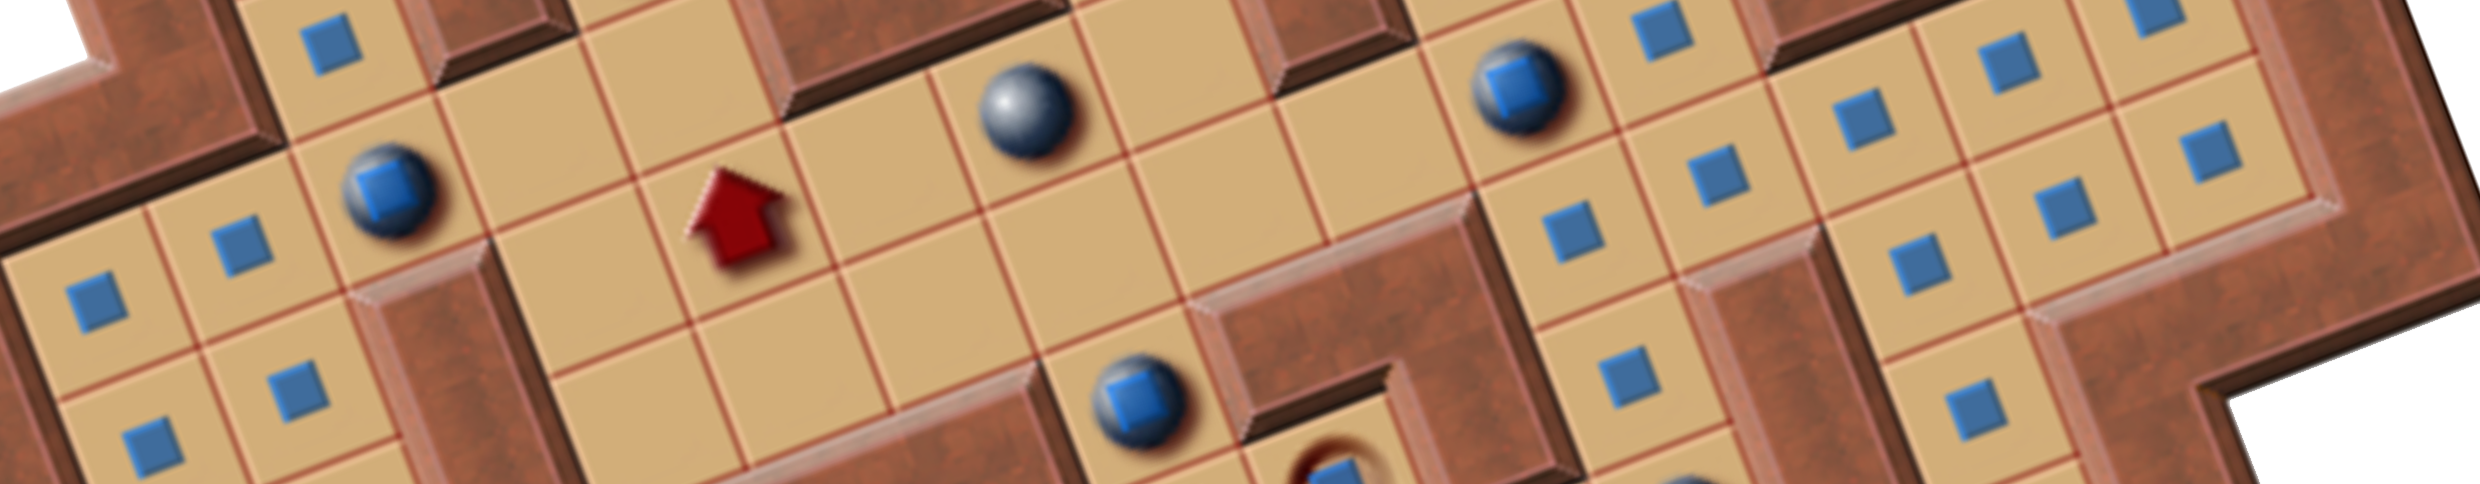
\includegraphics[width=\textwidth]{teaser}
  \caption{Sokoban level from the original game, released by Thinking Rabbit in 1982.}
  \label{fig:teaser}
\end{teaserfigure}

%%
%% This command processes the author and affiliation and title
%% information and builds the first part of the formatted document.
\maketitle

\section{Introduction}
Systems that exhibit probabilistic behaviour exist everywhere: computer networks, security protocols, and traffic flows, among others. Using probabilistic model checking, a technique used to verify the correctness of a model of a stochastic system, one can compute bounds on the likelihood that a state will be reached. This can help prevent undesirable behaviour, such as a system crash or a deadlock. As these systems get more complex, it is important to use tools that can verify these models efficiently.

Sokoban is a puzzle game where a player pushes boxes into pre-defined locations. Solving Sokoban levels has been proven to be an NP-hard problem \cite{sokoban-np}. Introducing stochastic behaviour into this game will allow for the game to be used to benchmark probabilistic model checking tools. This is done by defining a probability that determines how often the model checker deviates from the shortest solution.

The goal of this research is to generate probabilistic models from Sokoban levels in various formats so that these models can be used as part of a more extensive test suite to benchmark existing probabilistic model checking tools in competitions such as QComp\footnote{\url{https://qcomp.org/}}.


\section{Background}
\subsection{Sokoban}
Sokoban is a single-player transport puzzle game where the player pushes boxes around into predetermined locations. A level is completed when all boxes are pushed into the correct spots. The player can move and push boxes in 4 directions: up, down, left and right, and is contained by walls surrounding the level. \autoref{fig:sokoban} shows an example of a simple Sokoban level. Not only is solving Sokoban puzzles NP-hard, but it is also proven to be PSPACE-complete\cite{pspace-complete}, making it significantly more difficult to solve than many other NP-hard problems. As a result, there exist many levels that state-of-the-art solvers cannot solve. 

\begin{figure}[h]
    \centering
    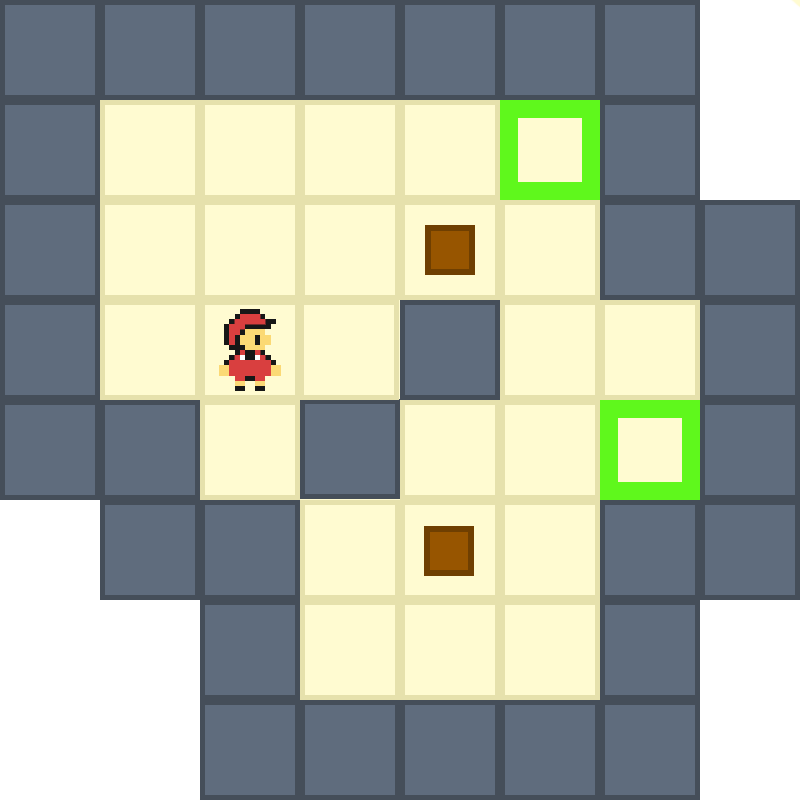
\includegraphics[width=5cm]{sokoban}
    \caption{An example Sokoban level. The gray tiles represent walls, the brown tiles represent boxes, and the green tiles are the targets.}
    \label{fig:sokoban}
\end{figure}

\subsection{Probabilistic model checking}
Model checking is a way of verifying the correctness of requirements of models. These models are often represented as finite-state machines. Using model checking tools, one can run queries on these state machines to verify the correctness of certain aspects of the model. A model of a Sokoban level would include the player and box positions, and the solution can be found by querying a state where all boxes are in the solved position. Probabilistic model checking is a similar technique that allows for verifying properties of models that exhibit stochastic behaviour. An example of such a model would be the model of a Sokoban level, but all inputs are randomly determined. One can now query the probability that the model ends up in an unsolvable state (e.g a box is pushed in a corner and can no longer move) or what the average length is to complete the level.

\subsection{Sok format}
.sok files\footnote{\url{http://www.sokobano.de/wiki/index.php?title=Sok_format}} are files that contain Sokoban levels. There are currently tens of thousands of user-created levels in this format freely available online. Apart from a few inconsistencies, the format is easy to parse and the large selection of levels makes it a good choice for this research. The contents of a .sok-file is depicted in \autoref{fig:sok}.

\lstset{basicstyle=\footnotesize\ttfamily,breaklines=true}

\begin{figure}[h]
    \subfloat[\centering ASCII representation of a .sok-file. '@' represents the player, '\$' represents a box, '.' represents a target location, and '\#' represents a wall.\label{fig:sok_ascii}]{\makebox[0.5\linewidth][c]{\lstinputlisting{code/level.sok}}}
    \hfill
    \subfloat[\centering Graphical representation of a .sok-file. The brown tiles represent boxes, the green tiles represent target locations, and the tiles blocks represent walls.]{\makebox[0.5\linewidth][c]{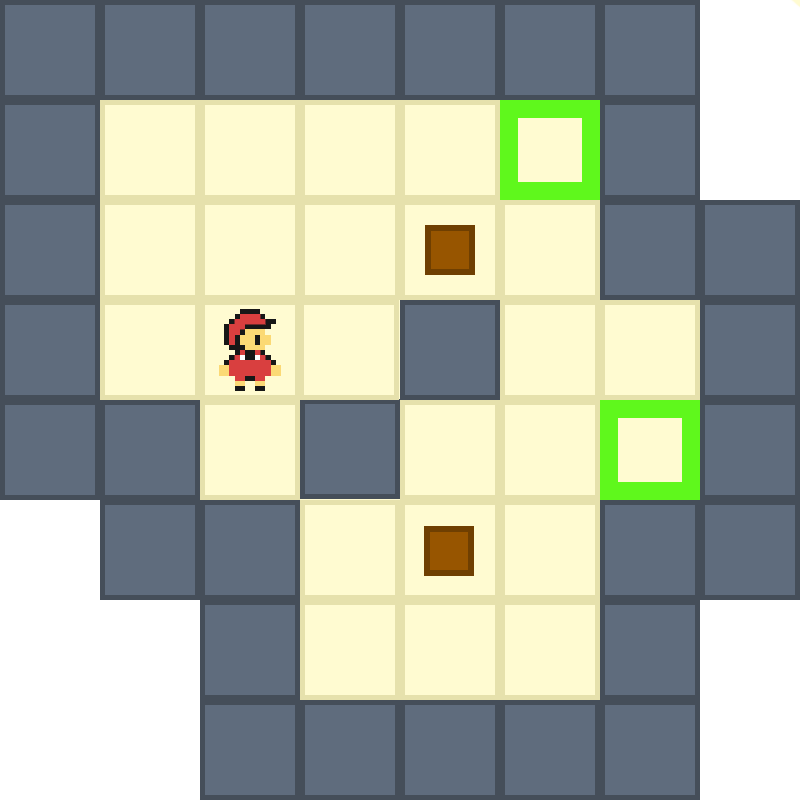
\includegraphics[width=3.5cm,valign=c]{sokoban.png}}}
    \caption{A .sok-file in both its ASCII and graphical representation.}
    \label{fig:sok}
\end{figure}


\section{Research questions}
\begin{enumerate}
    \item[\textbf{RQ1}.] To what extent do the stochastic additions influence the solutions generated by the model checker?
    \item[\textbf{RQ2}.] On average, which of the three model checkers, Storm, Modest, and PRISM, is the best suited for solving probabilistic Sokoban models?
\end{enumerate}

\section{Related work}
There exist many Sokoban solvers, such as Festival\footnote{\url{https://festival-solver.site/}} and Sokolution\footnote{\url{http://codeanalysis.fr/sokoban/}}. The goal of this research however is not to create a solver for (a stochastic version of) Sokoban, but to create a model that will be solved by a model checker.

A project similar to this research has been implemented that generates Sokoban models, which are then used to benchmark three different model checking tools: LTSmin, DiVinE and nuXmv\cite{comparing_sokoban}. It solely researched non-stochastic models, whereas this research only considers stochastic models and probabilistic model checking tools. While there was a comparison between a simple and more optimized model in that research, there was no attempt to find the optimal encoding of the player and box positions like there is in this research.

Similarly, another project focuses on generating models for various logic puzzles, including Sokoban, for LTSmin\cite{ltsmin-puzzles}. This research is different from the mentioned project for the same reasons as mentioned above.


\section{Method}
The research consists of two parts: (a) generating probabilistic models from existing Sokoban levels and a set of probabilities, and (b) experimenting with the generated models. 

For part a., stochastic behaviour has to be introduced to the non-stochastic game Sokoban. This is done by defining the following probabilities:
\begin{enumerate}
    \item The probability that decides if the player's move is respected, or if a different move is selected. Additionally, probabilities for each movement direction are defined.
    \item The probability that a box moves when not pushed by a player. Additionally, probabilities for each movement direction are defined.
\end{enumerate}

The probabilistic models are derived from .sok files, and the models are described by the PRISM language\cite{prism} and the JANI specification\cite{jani}, so that a wide range of probabilistic model checkers can be targetted. The goal is to create a tool that automates this process: using a .sok file and a set of probabilities as input, it should be able to output a probabilistic model in either the PRISM language, JANI, or both.

Additionally, the position of the player and the boxes are represented in multiple ways. Depending on how these values are encoded, the performance of the model checkers may differ.

The generated models abide by the following transition rules:
\begin{enumerate}
    \item The player can walk in any of the four directions (up, down, left, right) if:
    \begin{enumerate}
        \item there is not a box or wall at the destination. This action updates the player's position to the destination.
        \item there is a box at the respective destination and the tile behind the destination is not a wall nor box. This action moves the box one tile backwards, and updates the player's position to the destination.
    \end{enumerate}
\end{enumerate}

These transition rules do mean that it is possible to end up in unsolvable states: a player is able to position boxes in such a way that they can no longer push them, or they can lock themselves into an area of the level without being able to escape. However, with the stochastic additions it is possible that these situations resolve themselves eventually, whereas for the non-stochastic version of Sokoban one of those scenarios would most certainly require the player to reset from the start.


Part b. involves experimenting with the generated models using existing probabilistic modelling tools. The tests will be conducted in virtual machines with identical specifications running an identical operating system. This creates a consistent playing field for the model checkers so that the run time performance can be measured fairly. Depending on the duration of the tests, they will be run multiple times to reduce inconsistencies caused due to measurement errors. A test is deemed completed once the target state is reached.


% Part b. involves experimenting with the generated models using existing model checkers. Using these existing checkers, various stochastic properties can be verified about the models, such as:
% \begin{itemize}
%     \item The probability that a legal, unsolvable state is reached.
%     \item The probability that the target state is reached.
%     \item The probability that the target state is reached in less steps than the non-stochastic minimum solution.
% \end{itemize} 

% Additionally, during the generation phase, models can be generated in different ways. This may or may not improve performance for one or more checkers. By adding more constraints on what is and what is not considered a valid move, the state space can be reduced significantly. This can be done by disallowing moves that cause boxes to be stuck in corners or that moves that otherwise create an unsolvable state. These models will be referred to as the optimized models.

% Furthermore, 

% This yields the following research questions:
% \begin{enumerate}
%     \item What properties are interesting?
%     \todo[inline]{Poorly formulated RQ}
%     \item What is the effect of the optimization of the model on the run time and state space of the model checker?
% \end{enumerate}
% \todo[inline]{Something about model type?}
% \todo[inline]{Something about player/box position encoding?}

% \section{Method}
% A Sokoban level, in the sok format as depicted in \autoref{fig:sok_ascii}, is used as an input for a program. The program also requires a set of probabilities to be defined for the stochastic behaviour described in \autoref{sec:problem_statement}. It will output two models: one described in the PRISM language and one according to the JANI specification.

% For the regular models, the following transition rules are specified:
% \begin{itemize}
%     \item The player can walk in any of the four directions (up, down, left, right) if:
%     \begin{itemize}
%         \item there is not a box or wall at the destination. This action updates the player's position to the destination.
%         \item there is a box at the respective destination and the tile behind the destination is not a wall nor box. This action moves the box one tile backwards, and updates the player's position to the destination.
%     \end{itemize}
% \end{itemize}

% Additionally, for the optimized models the following rules are added:
% \begin{itemize}
%     \item A player may not push a box into a corner of the walls, unless this is required to reach the target state.
%     \item A player may not box themselves in by placing boxes in a way that they can no longer reach the target state.
% \end{itemize}
% Both these rules exist as there is no way to recover from these states. It is impossible to retrieve a box when it is placed in a corner, as a box can only be pushed from behind and the player is unable to phase through walls. When the level has multiple levels, in some cases it is possible that the player boxes themselves in by placing the boxes in such a way that their exit is cut off and they can no longer move the blocking boxes out of the way. By adding these two rules, it is possible that the state space will be reduced as there will be less solutions that end in an unsolvable state.

% The JANI model is run in mcsta, part of the Modest Toolset\footnote{\url{https://www.modestchecker.net/}}. The PRISM model is ran in PRISM. The tests will be conducted in virtual machines running Ubuntu 64-bit 20.04.4 LTS. Both machines have access to 1 CPU core, 20GB of storage space and 8 GB of RAM. This creates a consistent playing field for the model checkers so that run time performance can be measured fairly. Tests will be run 5 times and the run time will be averaged to smooth out any inconsistencies due to measurement errors. A test will be completed when the target state is reached, with a maximum time of 5 minutes before the test is deemed a failure.


\section{Planning}

The planning is described in \autoref{tab:project_deadlines} and \autoref{fig:project_goals}, the table describing the deadlines imposed by the module, and the figure describing the planning required to reach those deadlines.

\begin{table}[h]
\begin{tabular}{l|l}
\hline
Date      & Assignment/Task                   \\ \hline
8th May   & Final proposal submission         \\ \hline
10th May  & Proposal peer feedback submission \\ \hline
26th June & Draft paper submission            \\ \hline
3rd July  & Final paper submission            \\ \hline
8th July  & Conference presentation           \\ \hline
\end{tabular}
\caption{Research project deadlines for handing in assignments and doing tasks.}
\label{tab:project_deadlines}
\end{table}

\begin{figure}[h]
    \centering
    \begin{ganttchart}[y unit title=0.4cm,
y unit chart=0.5cm,
vgrid,hgrid, 
title label anchor/.style={below=-1.6ex},
title height=1,
progress label text={},
bar height=0.7,
group right shift=0,
group top shift=.6,
group height=.3]{1}{11}
%labels
\gantttitle{Week}{11} \\
\gantttitle{1}{1} 
\gantttitle{2}{1} 
\gantttitle{3}{1} 
\gantttitle{4}{1} 
\gantttitle{5}{1} 
\gantttitle{6}{1}
\gantttitle{7}{1} 
\gantttitle{8}{1} 
\gantttitle{9}{1} 
\gantttitle{10}{1} 
\gantttitle{11}{1} \\

%tasks
\ganttbar[bar/.append style={pattern=north east lines, pattern color=teal}]{Proposal}{1}{1}
\ganttbar[bar/.append style={pattern=north east lines, pattern color=teal}]{}{2}{2} \\
\ganttmilestone[milestone/.append style={fill=teal}]{Draft proposal}{1} \\
\ganttmilestone[milestone/.append style={fill=teal}]{Final proposal submission}{2} \\
\ganttbar[bar/.append style={pattern=north east lines, pattern color=orange}]{Implement project}{3}{5} \\
\ganttbar[bar/.append style={pattern=north east lines, pattern color=red}]{Run tests}{5}{6} \\
\ganttbar[bar/.append style={pattern=north east lines, pattern color=pink}]{Analyse measurements}{6}{7} \\
\ganttbar[bar/.append style={pattern=north east lines, pattern color=cyan}]{Write paper}{3}{9}
\ganttbar[bar/.append style={pattern=north east lines, pattern color=cyan}]{}{10}{10} \\
\ganttmilestone[milestone/.append style={fill=cyan}]{Draft paper submission}{9} \\
\ganttmilestone[milestone/.append style={fill=cyan}]{Final paper submission}{10} \\
\ganttbar[bar/.append style={pattern=north east lines, pattern color=lime}]{Prepare presentation}{10}{11} \\
\ganttmilestone[milestone/.append style={fill=lime}]{Conference}{11} \\

\end{ganttchart}
    \caption{Research project goals and milestones per week.}
    \label{fig:project_goals}
\end{figure}

%%
%% The next two lines define the bibliography style to be used, and
%% the bibliography file.
\bibliographystyle{ACM-Reference-Format}
\bibliography{bibliography}


\end{document}
\endinput
